\section{Sensor-space activity}

We computed average event-related fields (ERF) for each subject and sensor region.
Activity from these ERF was selected with two different types of time windows.

A positive effect indicates that activity evoked by object-relative clauses was more positive than activity evoked by subject-relative clauses. In the case of gradiometers, "more positive" means a higher regional RMS. With localized data, "more positive" means a higher z-score from the sLORETA source reconstruction.


\subsection{Interval analysis}
For this analysis, sensor activity from separate regions and hemispheres was compared blindly between 0 and 2200ms after onset in 200ms intervals.

After FDR-correction for 10 comparisons, no sensor region showed any non-spurious effect in either group ($p > 3\%$).

\subsection{Cluster analysis}
For this analysis, activity was compared between conditions using a temporal cluster analysis.

For children, significant differences were observed in the following sensor groups:
Right parietal magnetometers showed a negative effect between 159ms and 374ms ($p = 1.4\%$).
Left frontal magnetometers showed a negative effect between 375ms and 666ms ($p = 1.8\%$).
Left temporal magnetometers showed a negative effect between 349ms and 627ms ($p = 0.8\%$).
Right temporal gradiometers showed a positive effect between 1384ms and 1663ms ($p = 3.8\%$).
This activity can be summarized into two time windows: a negative effect between 159ms and 666ms, and a positive effect between 1426ms and 1663ms.

\begin{figure}[h]
\begin{center}
\vspace{7mm}
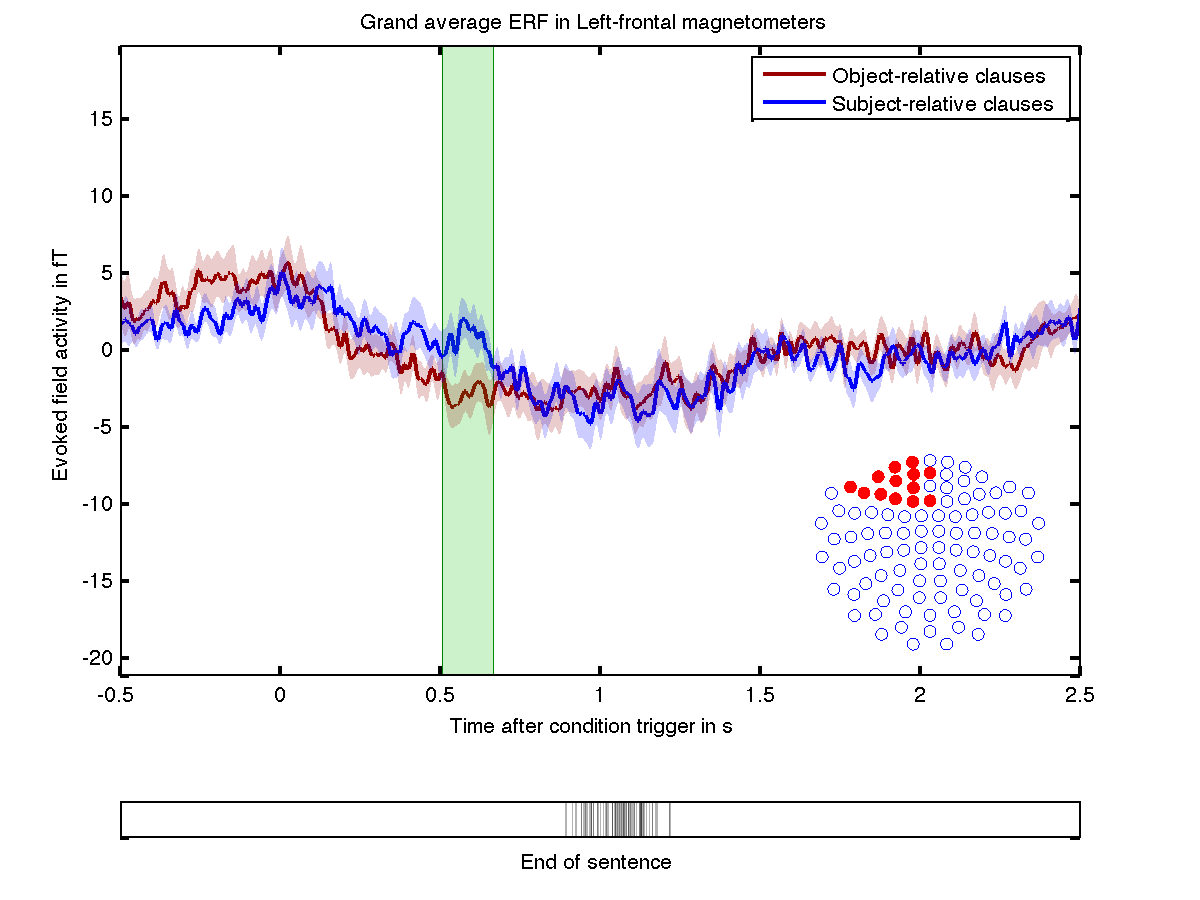
\includegraphics[width=0.49\textwidth]{pics/children_Left-frontal-magnetometers.png}
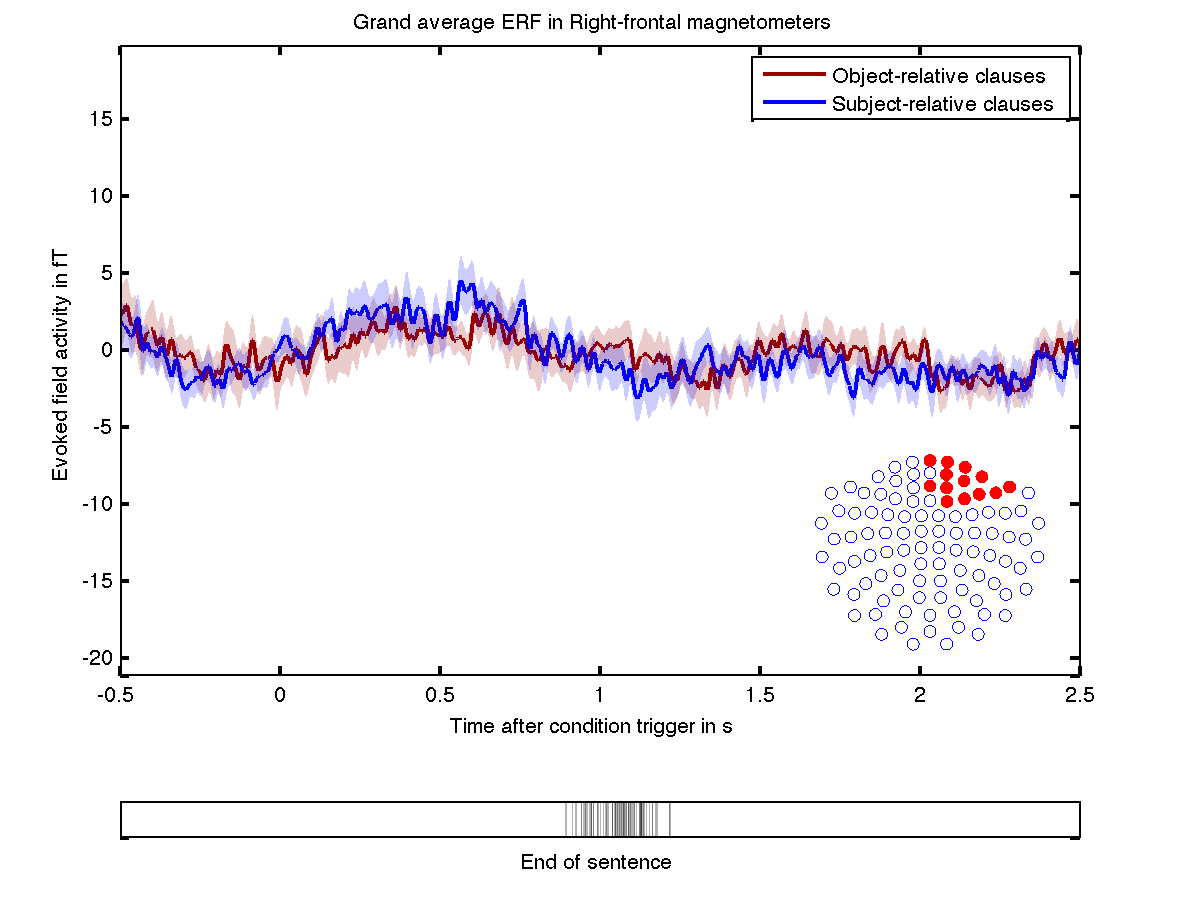
\includegraphics[width=0.49\textwidth]{pics/children_Right-frontal-magnetometers.png}
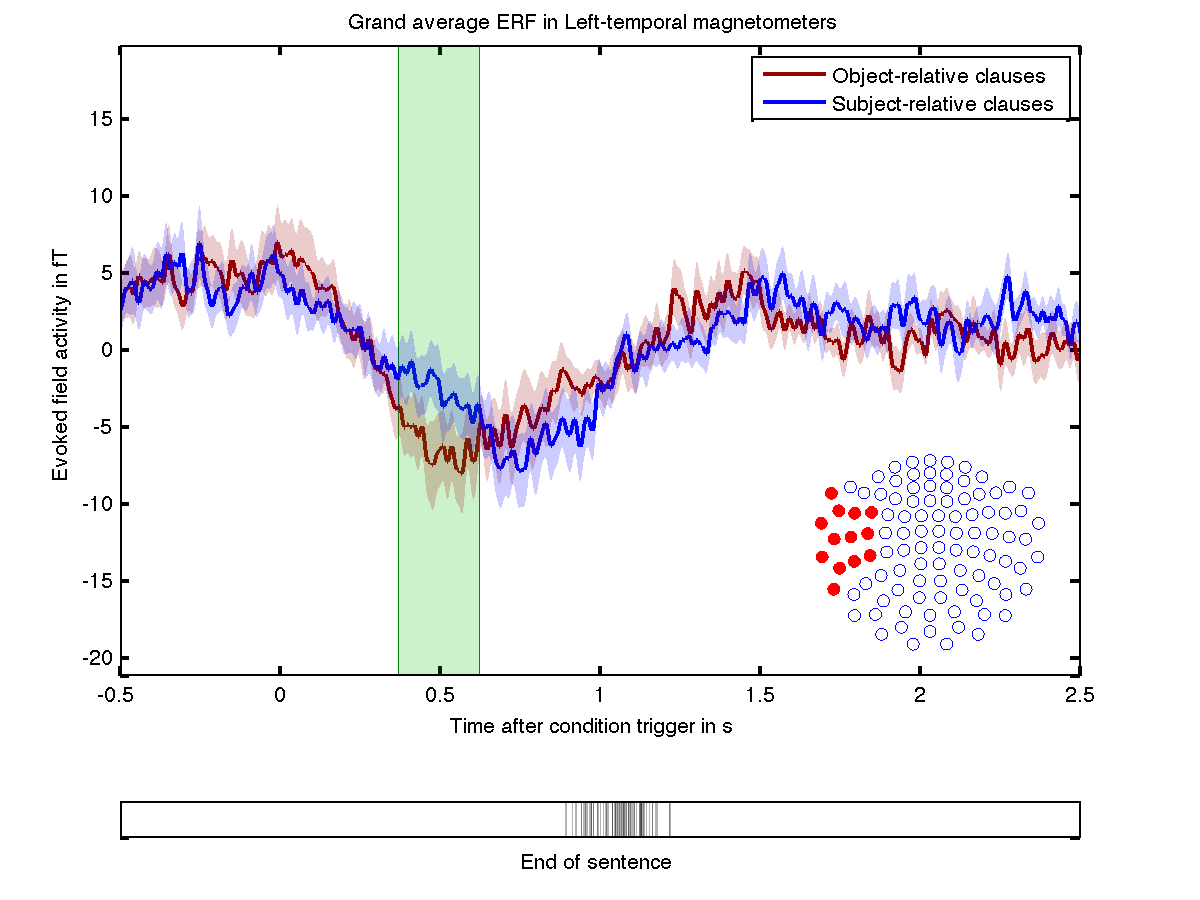
\includegraphics[width=0.49\textwidth]{pics/children_Left-temporal-magnetometers.png}
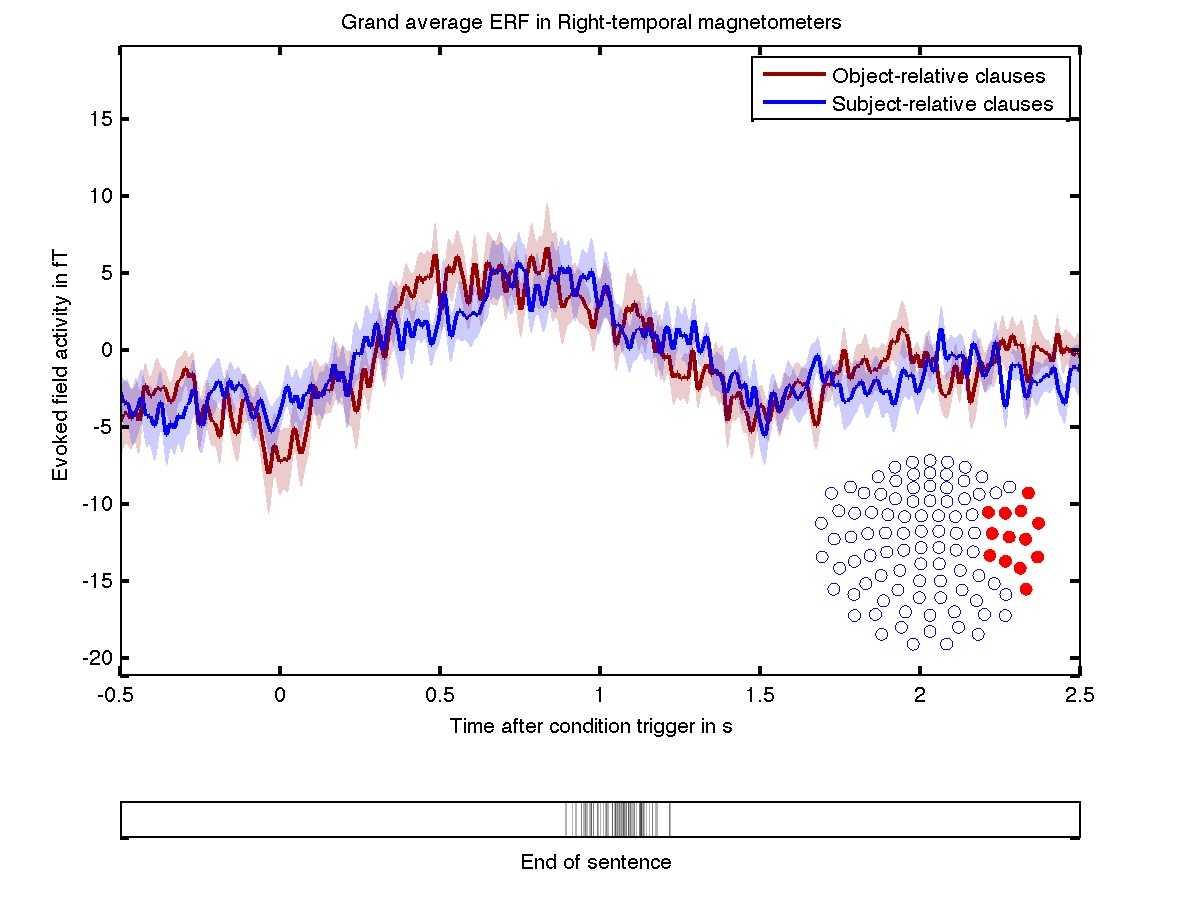
\includegraphics[width=0.49\textwidth]{pics/children_Right-temporal-magnetometers.png}
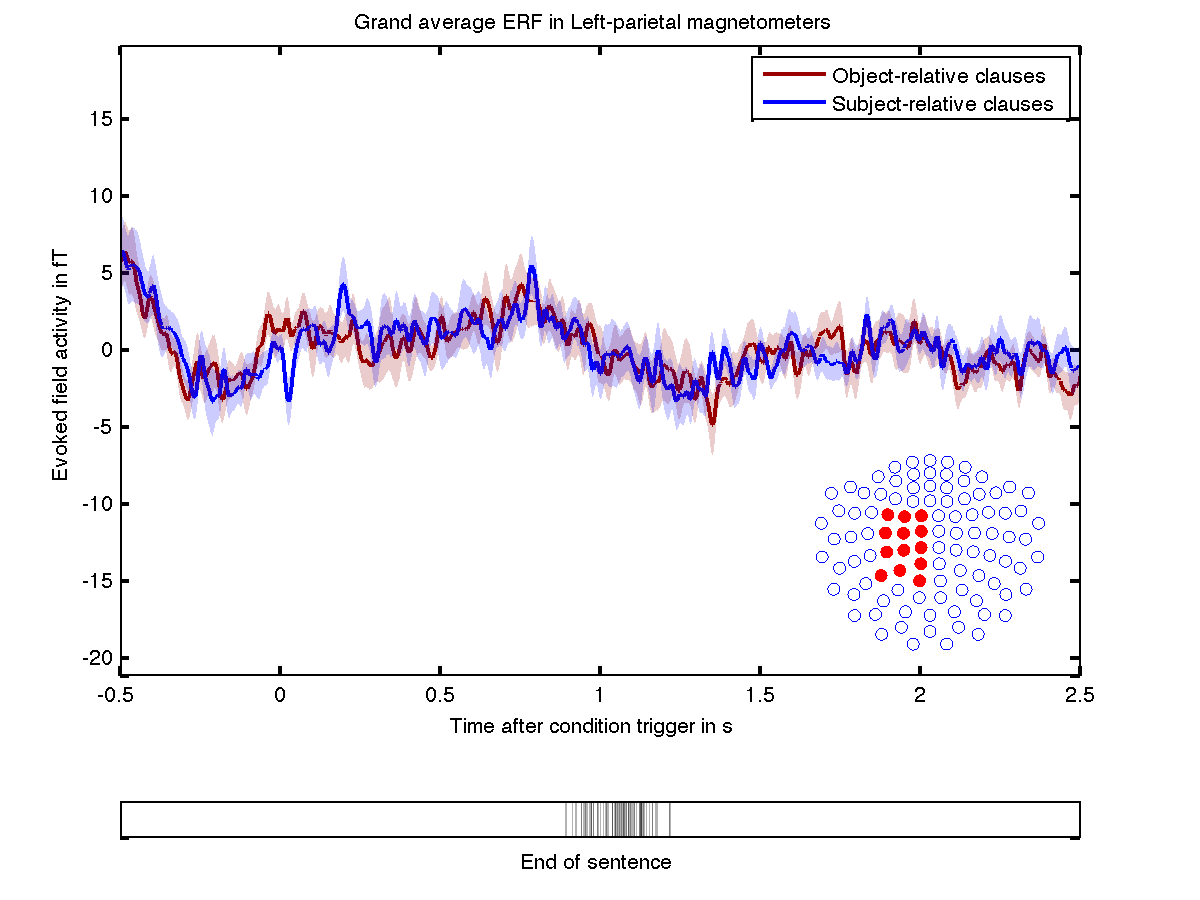
\includegraphics[width=0.49\textwidth]{pics/children_Left-parietal-magnetometers.png}
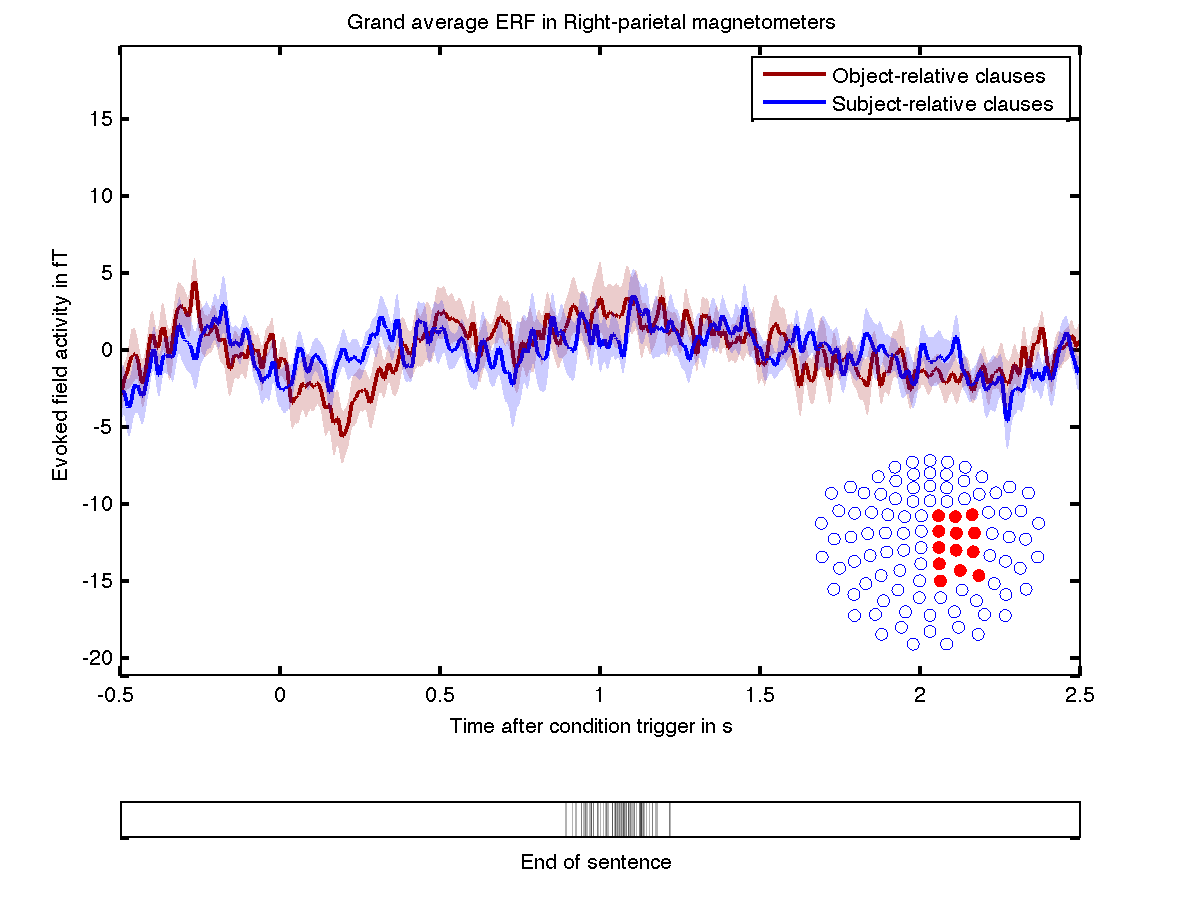
\includegraphics[width=0.49\textwidth]{pics/children_Right-parietal-magnetometers.png}
\caption{\label{4.2.activity.kids} Combined activity from children in separate sensor groups. Only magnetometers are displayed. Top: frontal sensor activity; middle: temporal sensor activity; bottom: parietal sensor activity}
\end{center}
\end{figure}

For adults, clusters of significant differences were observed by left-temporal gradiometers and left-parietal magnetometers.
Left frontal gradiometers showed a weak positive effect between 131ms and 284ms ($p = 6.3\%$).
Left temporal gradiometers showed a positive effect between 257ms and 480ms ($p = 2.1\%$).
Left parietal magnetometers showed a positive effect between 618ms and 765ms ($p = 0.64\%$).
Right temporal magnetometers showed a weak negative effect between 992 and 1154ms ($p = 7.1\%$).
This activity can be roughly categorized into three time windows: two positive effects between 131 and 480ms, 618 and 765ms, and a negative effect between 992 and 1154ms.
The generally lower significance levels imply an overall weaker impact of syntactic condition on sensor activity.

\begin{figure}[h]
\begin{center}
\vspace{7mm}
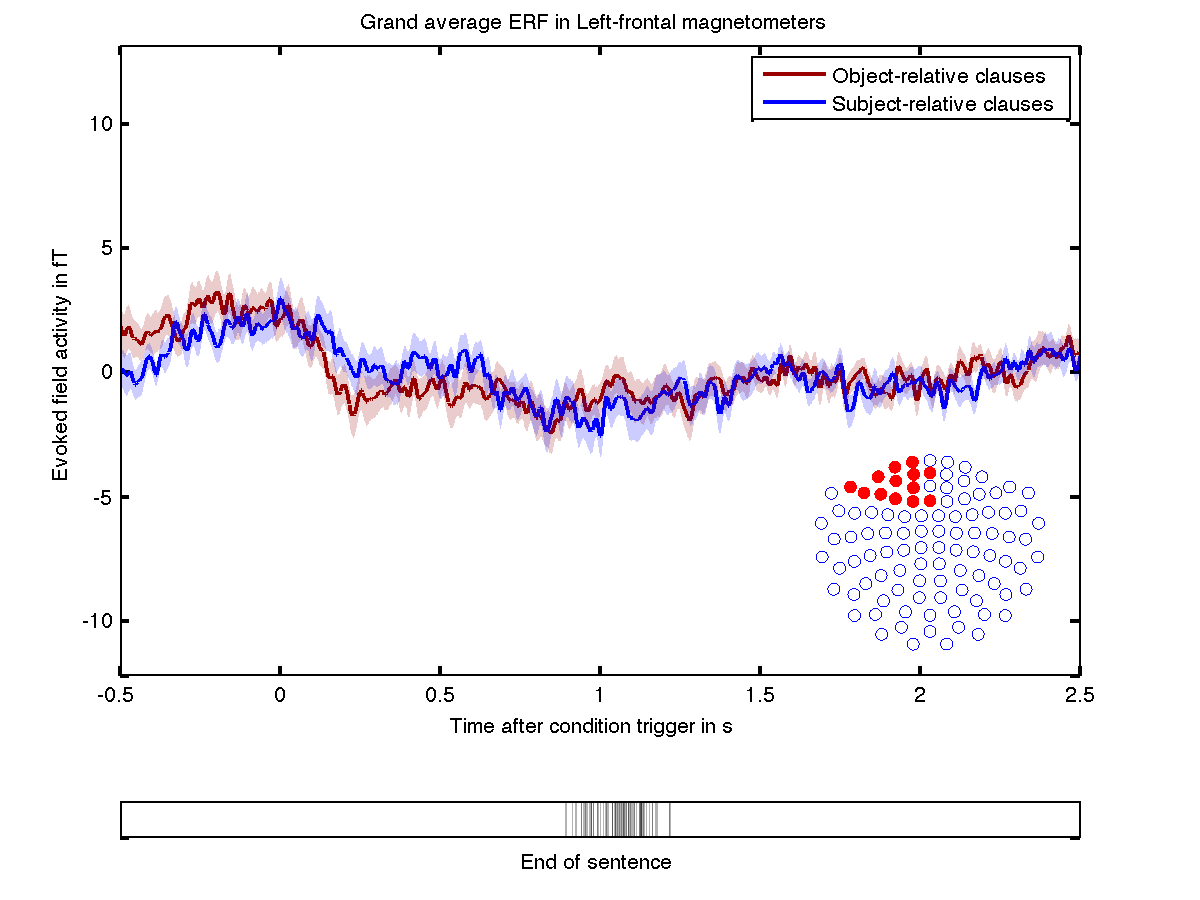
\includegraphics[width=0.49\textwidth]{pics/adults_Left-frontal-magnetometers.png}
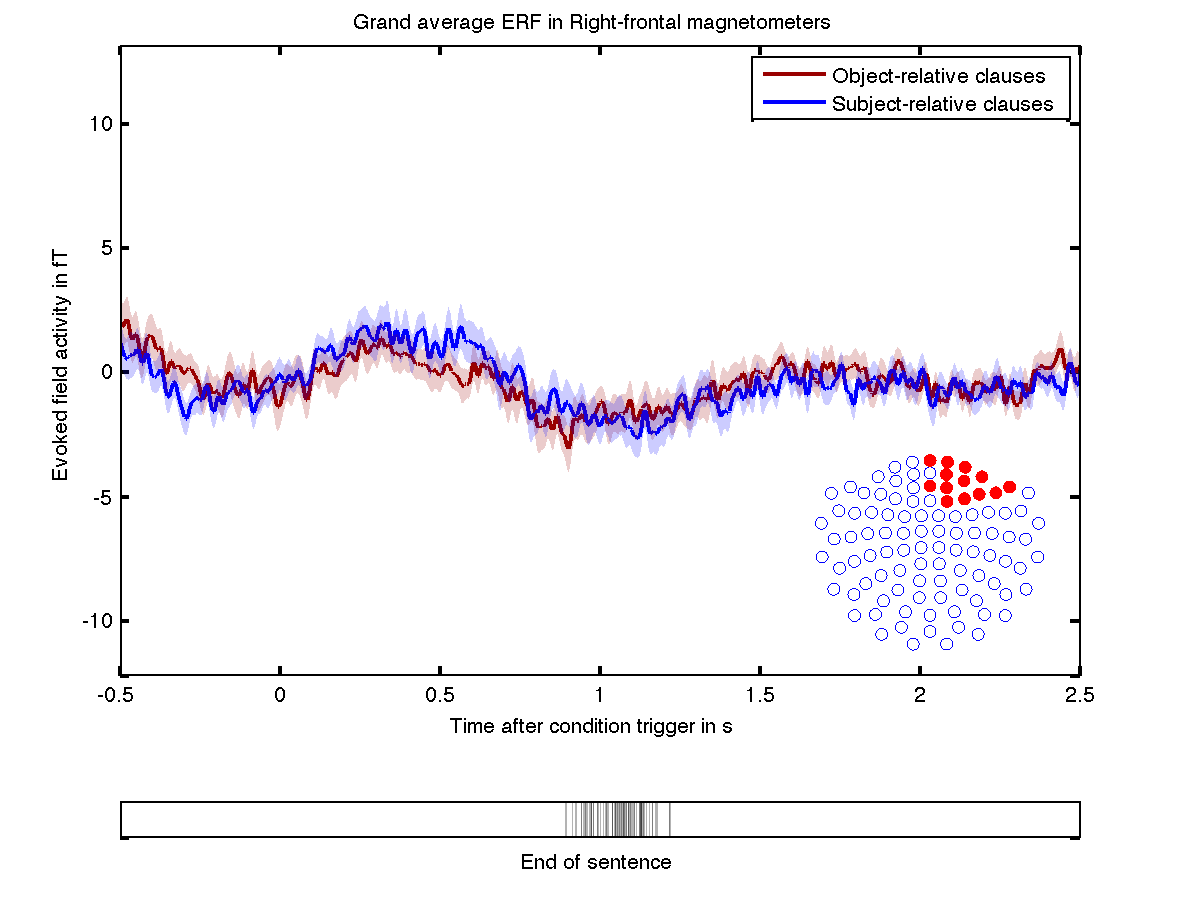
\includegraphics[width=0.49\textwidth]{pics/adults_Right-frontal-magnetometers.png}
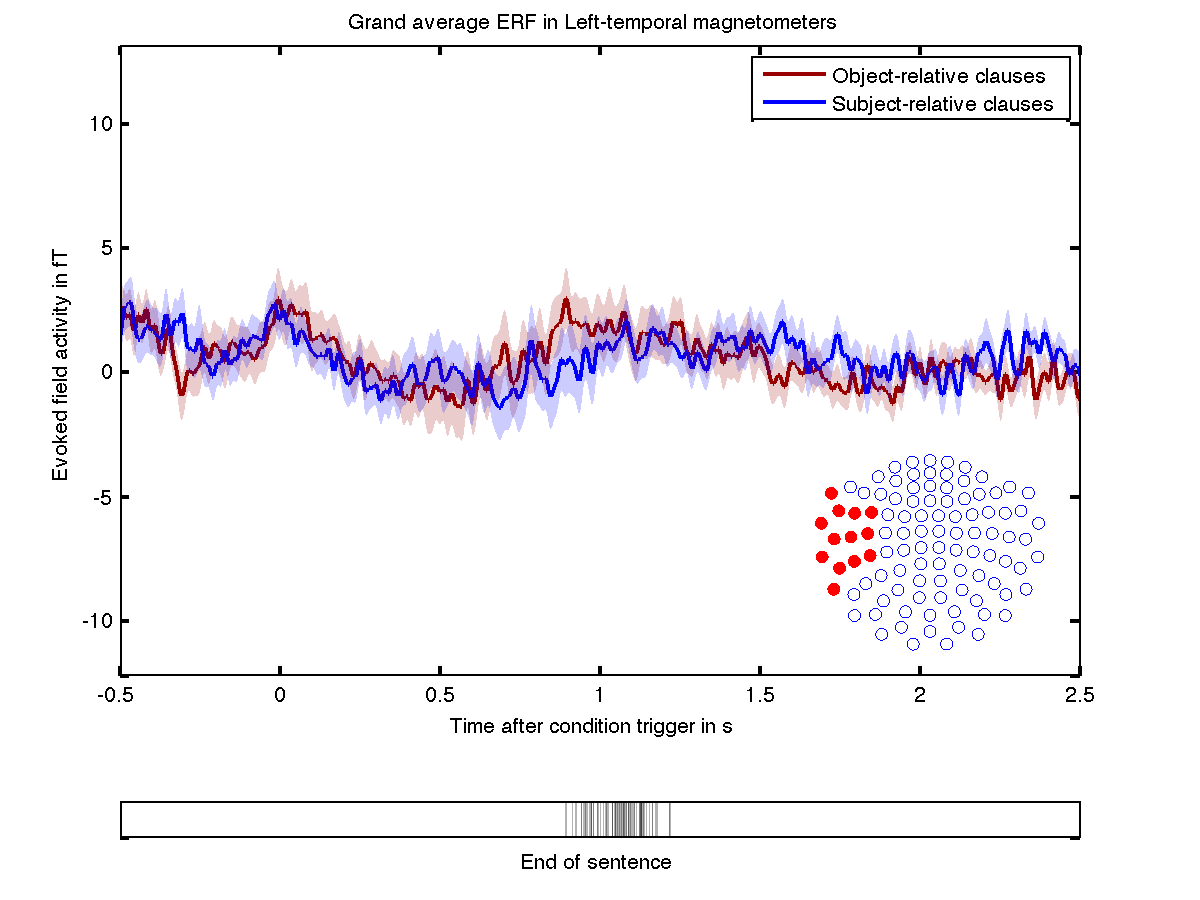
\includegraphics[width=0.49\textwidth]{pics/adults_Left-temporal-magnetometers.png}
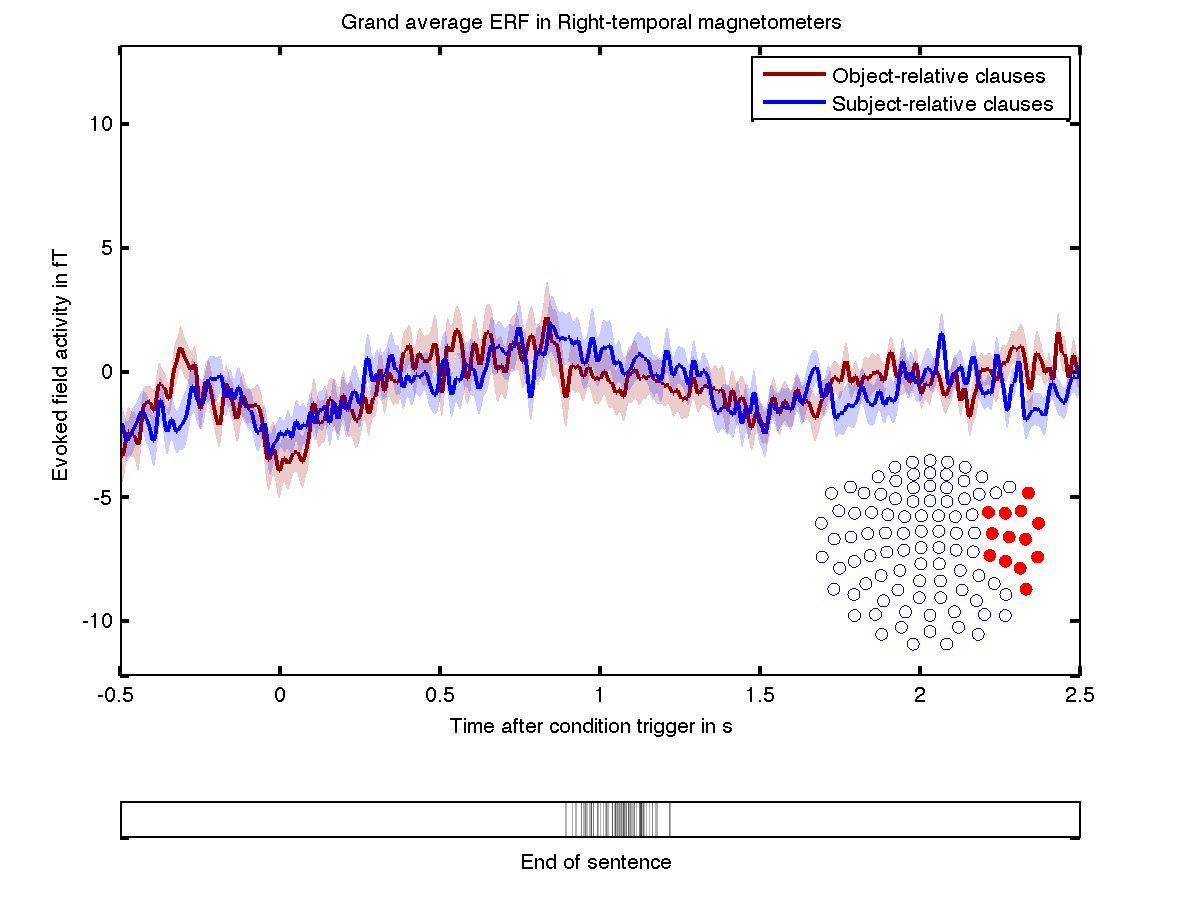
\includegraphics[width=0.49\textwidth]{pics/adults_Right-temporal-magnetometers.png}
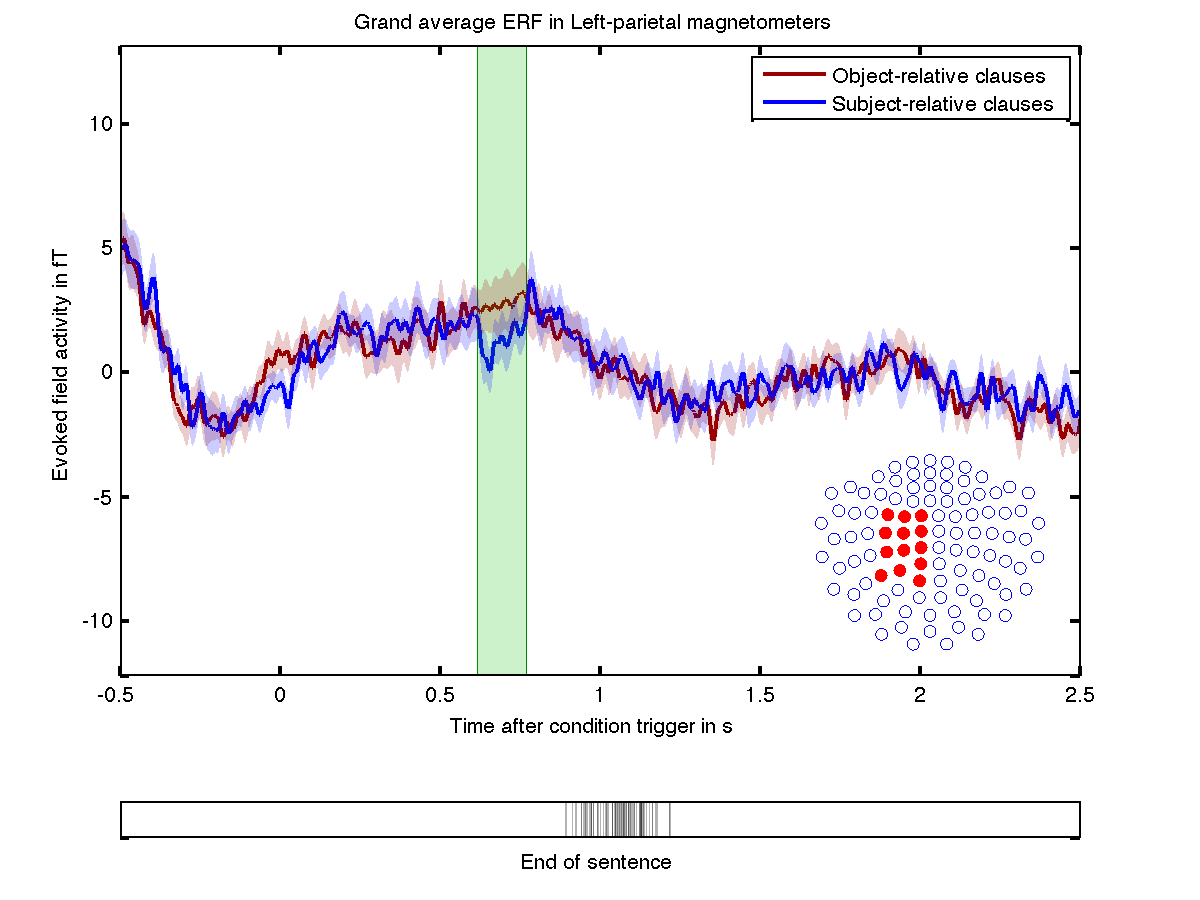
\includegraphics[width=0.49\textwidth]{pics/adults_Left-parietal-magnetometers.png}
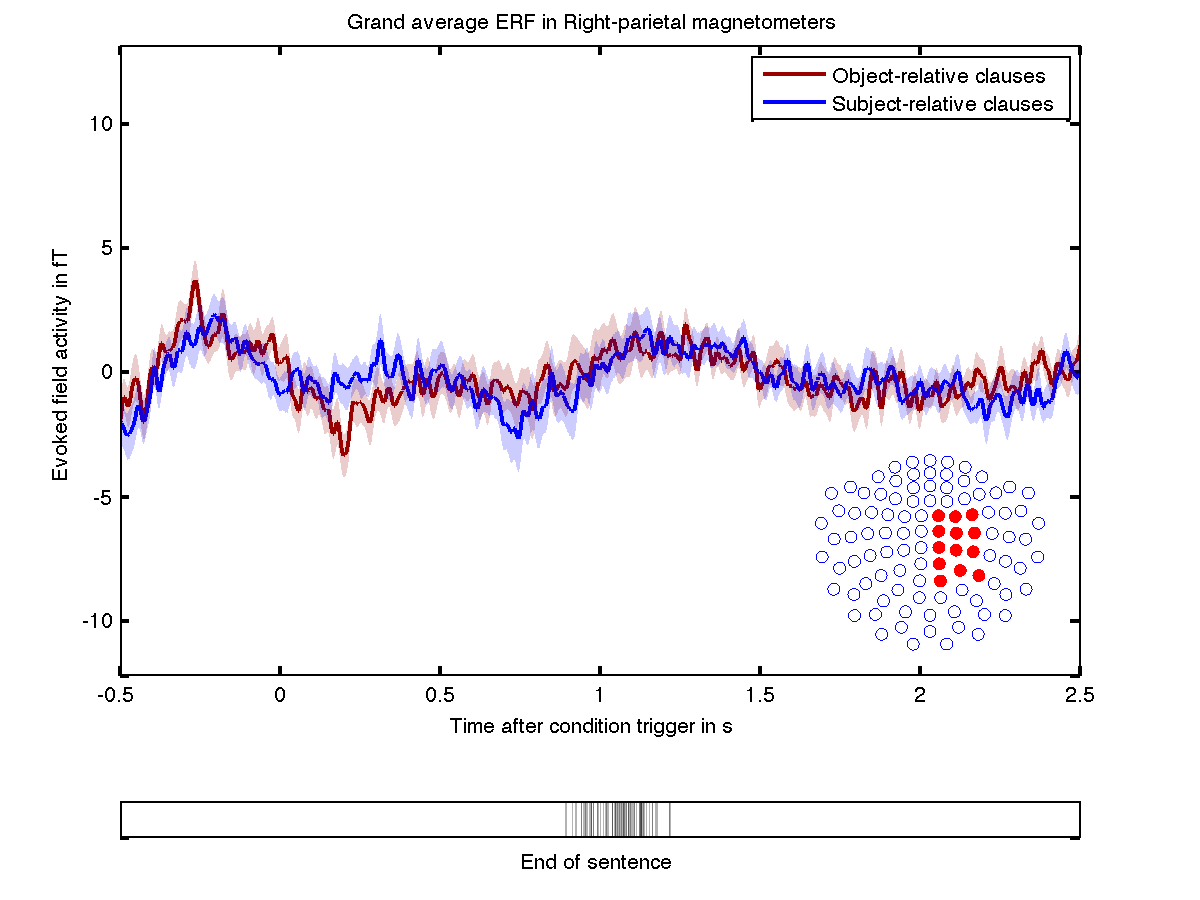
\includegraphics[width=0.49\textwidth]{pics/adults_Right-parietal-magnetometers.png}
\caption{\label{4.2.activity.adults} Combined activity from adults in separate sensor groups. Only magnetometers are displayed. Top: frontal sensor activity; middle: temporal sensor activity; bottom: parietal sensor activity}
\end{center}
\end{figure}